\subsection{Leptonic decays}

Purely leptonic decays of $\Dp$ and $\dsp$ mesons are among the simplest and theoretically cleanest
probes of $c\to d$ and $c\to s$ quark flavor-changing transitions. The branching fraction of leptonic 
decays that proceed via the annihilation of the initial quark-antiquark pair ($c\overline{d}$ or 
$c\overline{s}$) into a virtual $W^+$ that finally materializes as an antilepton-neutrino pair ($\ellnu$) is 
given in the Standard Model by
\begin{equation}
 \br(D_{q}^+\to \ell^+\nu_{\ell})=\frac{G_F^2}{8\pi}\tau_{D_q}f_{D_{q}}^2|V_{cq}|^2m_{D_{q}}m_{\ell}^2\left(1-\frac{m_{\ell}^2}{m_{D_{q}}^2} \right)^2.
 \label{eq:brCharmLeptonicSM}
\end{equation}
Here, $m_{D_{q}}$ is the $D_{q}$ meson mass, $\tau_{D_q}$ is its lifetime, $m_{\ell}$ is the charged lepton mass, 
$|V_{cq}|$ is the magnitude of the relevant CKM matrix element, and $G_F$ is the Fermi coupling constant. The parameter 
$f_{D_{q}}$ is the $D_q$ meson decay constant and is related to the wave-function overlap of the meson's 
constituent quark and anti-quark. Within the SM, the decay constants have been predicted using several 
methods, the most precise being the lattice gauge theory (LQCD) calculations. The Flavor Lattice Averaging 
Group~\cite{FLAG} combines all LQCD calculations and provides averaged values for $f_D$ and $f_{D_s}$ (see 
Table~\ref{tab:Lattice}) that are used within this section to extract the magnitudes of the $V_{cd}$ and $V_{cs}$ CKM
matrix elements from experimentally measured branching fractions of $D^+\to \ell^+\nu_{\ell}$ and 
$D_s^+\to \ell^+\nu_{\ell}$ decays, respectively.
\begin{table}[b!]
\caption{The LQCD average for $D$ and $D_s$ meson decay constants and their ratio from the Flavor Lattice Averaging 
Group~\cite{FLAG}.
\label{tab:Lattice}}
\begin{center}
\begin{tabular}{ll}
\toprule
\rowcolor{Gray} Quantity & Value \\ 
\midrule
$f_D$ 		& $209.2\pm3.3$~MeV\\
$f_{D_s}$ 	& $248.6\pm2.7$~MeV\\
$f_{D_s}/f_D$	& $1.187\pm0.012$
\\ \bottomrule
\end{tabular}
\end{center}
\end{table}


The leptonic decays of pseudoscalar mesons 
are suppressed by helicity conservation and their decay rates are thus proportional to the square of 
the charged lepton mass. Leptonic decays into electrons with $\br\lesssim 10^{-7}$ are not experimentally 
observable yet whereas decays to taus are favored over decays to muons. In particular, the ratio of the 
latter decays is equal to 
$R^{D_q}_{\tau/\mu}\equiv \br(D^+_q\to\tau^+\nu_{\tau})/\br(D^+_q\to\mu^+\nu_{\mu})=m_{\tau}^2/m_{\mu}^2\cdot(1-m^2_{\tau}/m^2_{D_q})^2/(1-m^2_{\mu}/m^2_{D_q})^2=9.76\pm0.03$ 
in the case of $D_s^+$ decays and to $2.67\pm0.01$ in the case of $D^+$ decays based on the world average values of masses of the muon, tau and 
$D_q$ meson given in Ref.~\cite{PDG_2012}. 
Any deviation from this expectation could only be interpreted as violation of lepton universality in charged 
currents and would hence point to NP effects~\cite{Filipuzzi:2012mg}.

Averages presented within this subsection are weighted averages and correlations between measurements and dependencies on input parameters
are taken into account.

\subsubsection{$D^+\to \ell^+\nu_{\ell}$ decays and $|V_{cd}|$}

We use measurements of the branching fraction $\br(D^+\to\munu)$ from \mbox{CLEO-c}~\cite{Eisenstein:2008aa} and 
BESIII~\cite{Ablikim:2013uvu} to calculate its world average (WA) value. We obtain
\begin{equation}
 \br^{\rm WA}(D^+\to\munu) = (3.74\pm0.17)\times10^{-4},
 \label{eq:Br:WA:DtoMuNu}
\end{equation}
from which we determine the product of the decay constant and the CKM matrix element to be
\begin{equation}
 f_{D}|V_{cd}| = \left(45.9\pm1.1\right)~\mbox{MeV},
 \label{eq:expFDVCD}
\end{equation}
where the uncertainty includes the uncertainty on $\br^{\rm WA}(D^+\to\munu)$ and external inputs\footnote{These values (taken from the PDG~\cite{PDG_2012}) are
$m_{\mu} = (0.1056583715\pm0.0000000035)$~GeV/$c^2$, $m_D = (1.86962\pm0.00015)$~GeV/$c^2$ 
and $\tau_D = (1040\pm7)\times 10^{-15}$~s.} needed to extract $f_{D}|V_{cd}|$ from the 
measured branching fraction using Eq.~\ref{eq:brCharmLeptonicSM}. 
Using the LQCD value for $f_D$ from Table~\ref{tab:Lattice} we 
finally obtain the CKM matrix element $V_{cd}$ to be
\begin{equation}
 |V_{cd}| = 0.219\pm0.005(\rm exp.)\pm0.003(\rm LQCD),
 \label{eq:Vcd:WA:Leptonic}
\end{equation}
where the uncertainties are from the experiments and lattice calculations, respectively. All input values
and the resulting world averages are summarized in Table~\ref{tab:DExpLeptonic} and plotted in 
Fig.~\ref{fig:ExpDLeptonic}.
\begin{table}[t!]
\caption{Experimental results and world averages for ${\cal{B}}(D^+\to \ell^+\nu_{\ell})$ and $f_{D}|V_{cd}|$.
The first uncertainty is statistical and the second is experimental systematic. The third uncertainty in the case
of $f_{D^+}|V_{cd}|$ is due to external inputs (dominated by the uncertainty of $\tau_D$).
\label{tab:DExpLeptonic}}
\begin{center}
\begin{tabular}{lccll}
\toprule
\rowcolor{Gray} Mode 	& ${\cal{B}}$ ($10^{-4}$)	& $f_{D}|V_{cd}|$ (MeV)		& Reference & \\ 
\midrule
% this is from floated taunu fit
%$\munu$		& $3.93\pm0.35\pm 0.09$ 	& $???.?\pm?.?\pm?.?$	& CLEO-c\hfill \cite{Eisenstein:2008aa}\\
% this is from fixed taunu contribution fit (same for BESIII)
\multirow{2}{*}{$\munu$} & $3.82\pm0.32\pm 0.09$ 	& $46.4\pm1.9\pm0.5\pm0.2$	& CLEO-c & \cite{Eisenstein:2008aa}\\ 
			& $3.71\pm0.19\pm 0.06$ 	& $45.7\pm1.2\pm0.4\pm0.2$	& BESIII & \cite{Ablikim:2013uvu}\\
\midrule
\rowcolor{Gray}$\munu$ 	& $3.74\pm0.16\pm 0.05$		& $45.9\pm1.0\pm0.3\pm0.2$	& Average & \\
\midrule
$\enu$	 		& {$<0.088$ at 90\% C.L.}	&& CLEO-c & \cite{Eisenstein:2008aa}\\
\midrule
$\taunu$ 		& {$<12$ at 90\% C.L.}		&& CLEO-c & \cite{Eisenstein:2008aa}
\\ \bottomrule
\end{tabular}
\end{center}
\end{table}
\begin{figure}[hbt!]
\centering
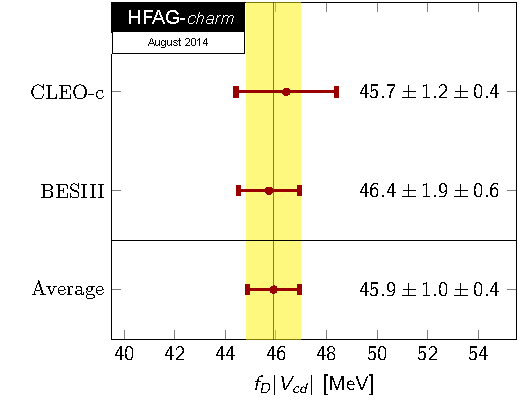
\includegraphics[width=0.7\textwidth]{figures/charm/fDVcd.pdf}
\caption{
WA value for $f_{D}|V_{cd}|$. For each point, the first error listed is the statistical and the second error is the systematic error.
\label{fig:ExpDLeptonic}
}
\end{figure}
 
The upper limit on the ratio of branching fractions is found to be $R_{\tau/\mu}^D<3.2$ at 90\%~C.L., which is just slightly above the SM expected value, $2.67\pm0.01$.

\subsubsection{$D_s^+\to \ell^+\nu_{\ell}$ decays and $|V_{cs}|$}

We use measurements of the absolute branching fraction $\br(D_s^+\to\munu)$ from CLEO-c~\cite{Alexander:2009ux}, \babar~\cite{delAmoSanchez:2010jg},
and Belle~\cite{Zupanc:2013byn} and obtain a WA value of
\begin{equation}
 \br^{\rm WA}(\dsmunu) = (5.57\pm0.24)\times10^{-3}.
 \label{eq:Br:WA:DstoMuNu}
\end{equation}
The WA value for $\br(D_s^+\to\taunu)$ is also calculated from CLEO-c, \babar, and Belle measurements. 
CLEO-c made separate measurements for $\tau^+\to e^+\nu_e\overline{\nu}{}_{\tau}$~\cite{Naik:2009tk},
$\tau^+\to\pi^+\overline{\nu}{}_{\tau}$~\cite{Alexander:2009ux}, and
$\tau^+\to\rho^+\overline{\nu}{}_{\tau}$~\cite{Onyisi:2009th};
\babar made separate measurements for 
$\tau^+\to e^+\nu_e\overline{\nu}{}_{\tau}$~\cite{delAmoSanchez:2010jg} and $\tau^+\to \mu^+\nu_{\mu}\overline{\nu}{}_{\tau}$; and
Belle made separate measurements for $\tau^+\to e^+\nu_e\overline{\nu}{}_{\tau}$, $\tau^+\to \mu^+\nu_{\mu}\overline{\nu}{}_{\tau}$, 
and $\tau^+\to\pi^+\overline{\nu}{}_{\tau}$~\cite{Zupanc:2013byn}.
Combining all of them we obtain the WA value of
\begin{equation}
 \br^{\rm WA}(\dsp\to\taunu) = (5.55\pm0.24)\times10^{-2}.
 \label{eq:Br:WA:DstoTauNu}
\end{equation}

The ratio of branching fractions is found to be
\begin{equation}
R_{\tau/\mu}^{\ds} = 9.96\pm0.57,
\label{eq:R:WA:Leptonic}
\end{equation}
and is consistent with the value expected in the SM, $9.76\pm0.03$.

From the average values of branching fractions of muonic and tauonic decays we determine\footnote{
We use the following values (taken from PDG~\cite{PDG_2012}) for external parameters entering 
Eq.~\ref{eq:brCharmLeptonicSM}: $m_{\tau} = (1.77682\pm0.00016)$~GeV/$c^2$, $m_{D_s} = (1.96850\pm0.00032)$~GeV/$c^2$ 
and $\tau_{D_s} = (500\pm7)\times 10^{-15}$~s.} the product of $D_s$ meson decay constant and 
the $|V_{cs}|$ CKM matrix element to be
\begin{equation}
 \fds|V_{cs}|=\left(250.6\pm4.5\right)~\mbox{MeV},
 \label{eq:expFDSVCS}
\end{equation}
where the uncertainty is due to the uncertainties on $\br^{\rm WA}(D_s^+\to\munu)$ and 
$\br^{\rm WA}(D_s^+\to\taunu)$ and the external inputs. All input values and the resulting world averages are 
summarized in Table~\ref{tab:DsLeptonic} and plotted in Fig.~\ref{fig:ExpDsLeptonic}. To obtain the 
averages given within this subsection and in Table~\ref{tab:DsLeptonic} we have taken into account
the correlations within each experiment\footnote{In the case of \babar we use the covariance matrix from 
the errata of~Ref.\cite{delAmoSanchez:2010jg}.} for the uncertainties related to: normalization, tracking, particle identification, 
signal and background parameterizations, and peaking background contributions.
% \end{itemize}

Using the LQCD value for $\fds$ from Table~\ref{tab:Lattice} we 
finally obtain the CKM matrix element $V_{cs}$ to be
\begin{equation}
 |V_{cs}| = 1.008\pm0.018(\rm exp.)\pm0.011(\rm LQCD),
 \label{eq:Vcs:WA:Leptonic}
\end{equation}
where the uncertainties are from the experiments and lattice calculations, respectively.

\begin{table}[t!]
\caption{Experimental results and world averages for ${\cal{B}}(\dsellnu)$ and $f_{D_s}|V_{cs}|$.
The first uncertainty is statistical and the second is experimental systematic. The third uncertainty 
in the case of $f_{D_s}|V_{cs}|$ is due to external inputs (dominated by the uncertainty of $\tau_{D_s}$).
We have recalculated $\br(\dsp\to\taunu)$ quoted by CLEO-c and \babar using the latest 
values for branching fractions of $\tau$ decays to electron, muon, or pion and neutrinos~\cite{PDG_2012}.
CLEO-c and \babar include statistical uncertainty of number of $\ds$ tags (denominator in the calculation of 
branching fraction) in the statistical uncertainty of measured $\br$. We subtract this uncertainty from the
statistical one and add it to the systematic uncertainty. 
\label{tab:DsLeptonic}}
\begin{center}
\begin{tabular}{lccll}
\toprule
\rowcolor{Gray}
Mode 		& ${\cal{B}}$ ($10^{-2}$) 	& $f_{D_s}|V_{cs}|$ (MeV) 		& Reference & 
\\ \midrule
\multirow{3}{*}{$\munu$}	& $0.565\pm0.044\pm 0.020$ 	& $250.8 \pm 9.8 \pm 4.4 \pm 1.8$	& CLEO-c &\cite{Alexander:2009ux}\\		
				& $0.602\pm0.037\pm 0.032$ 	& $258.9 \pm 8.0 \pm 6.9 \pm 1.8$	& \babar  &\cite{delAmoSanchez:2010jg}\\
				& $0.531\pm0.028\pm 0.020$ 	& $243.1 \pm 6.4 \pm 4.6 \pm 1.7$ 	& Belle  &\cite{Zupanc:2013byn}\\
\midrule
\rowcolor{Gray}
$\munu$ 			& $0.557\pm0.020\pm0.014$ 		& $249.0 \pm 4.5 \pm 3.1 \pm 1.7$ 	& Average & \\
\midrule
$\tauenu$ 			& $5.31\pm0.47\pm0.22$ 		& $246.1 \pm 10.9 \pm 5.1 \pm 1.7$ 	& CLEO-c &\cite{Onyisi:2009th}\\
$\taupinuCharm$ 			& $6.46\pm0.80\pm0.23$ 		& $271.4 \pm 16.8 \pm 4.8 \pm 1.9$  & CLEO-c &\cite{Alexander:2009ux}\\
$\taurhonu$ 			& $5.50\pm0.54\pm0.24$ 		& $250.4 \pm 12.3 \pm 5.5 \pm 1.8$  & CLEO-c &\cite{Naik:2009tk}\\
\midrule
\rowcolor{LightGray}
$\taunu$			& $5.57\pm0.32\pm0.15$		& $252.0 \pm 7.2 \pm 3.4 \pm 1.8$   & CLEO-c & \\
\midrule
$\tauenu$ 			& $5.08\pm0.52\pm0.68$ 		& $240.7 \pm 12.3 \pm 16.1 \pm 1.7$	& \multirow{2}{*}{\babar} & \multirow{2}{*}{\cite{delAmoSanchez:2010jg}}\\
$\taumunu$ 			& $4.90\pm0.46\pm0.54$ 		& $236.4 \pm 11.1 \pm 13.0 \pm 1.7$	&  & \\
\midrule
\rowcolor{LightGray}
$\taunu$			& $4.95\pm0.36\pm0.58$		& $237.6 \pm 8.6 \pm 13.8 \pm 1.7$   & \babar &\\
\midrule
$\tauenu$  			& $5.37\pm0.33^{+0.35}_{-0.31}$ & $247.4 \pm 7.6^{+8.1}_{-7.1} \pm 1.7$  & \multirow{3}{*}{Belle} & \multirow{3}{*}{\cite{Zupanc:2013byn}} \\
$\taumunu$ 		 	& $5.86\pm0.37^{+0.34}_{-0.59}$ & $258.5 \pm 8.2^{+7.5}_{-13.0} \pm 1.8$  & &\\ 
$\taupinuCharm$  			& $6.04\pm0.43^{+0.46}_{-0.40}$ & $262.4 \pm 9.3^{+10.0}_{-8.7} \pm 1.8$  & &\\
\midrule
\rowcolor{LightGray}
$\taunu$			& $5.70\pm0.21\pm0.31$		& $254.9 \pm 4.7 \pm 6.9 \pm 1.8$   & Belle & \\
\midrule
\rowcolor{Gray}
$\taunu$ 			& $5.55\pm0.18\pm0.17$ 		& $251.5 \pm 4.1 \pm 3.9 \pm 1.8$	& Average & \\
\midrule
\rowcolor{Gray}
$\munu$  			&		 		& \multirow{2}{*}{$250.6\pm 3.1\pm 2.8\pm1.8$}	& \multirow{2}{*}{Average} & \\
\rowcolor{Gray}
$\taunu$ 			&		 		& \multirow{-2}{*}{$250.6\pm 3.1\pm 2.8\pm1.8$}	& \multirow{-2}{*}{Average} & \\
\midrule
$\enu$				& $<0.0083$ at 90\% C.L.	& 					& Belle & \cite{Zupanc:2013byn} \\
\bottomrule
\end{tabular}
\end{center}
\end{table}
\begin{figure}[hbt!]
\centering
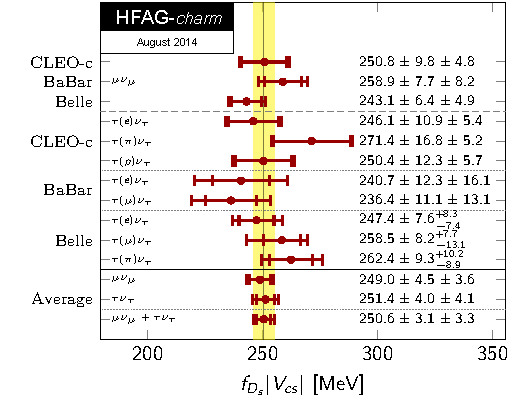
\includegraphics[width=1\textwidth]{figures/charm/fDsVcs.pdf}
\caption{
WA value for $f_{D_s}|V_{cs}|$. For each point, the first error listed is the statistical and the second error is the systematic error.
\label{fig:ExpDsLeptonic}
}
\end{figure}


\subsubsection{Comparison with other determinations of $|V_{cd}|$ and $|V_{cs}|$}

Table~\ref{tab:CKMVcdVcs} summarizes and Fig.~\ref{fig:VcdVcsComparions} shows all determinations of the CKM matrix elements $|V_{cd}|$ and $|V_{cs}|$. As
can be seen, the most precise direct determinations of these CKM matrix elements are those from leptonic and semileptonic $D_{(s)}$ decays. The values are in agreement
within uncertainties with the values obtained from the global fit assuming CKM matrix unitarity.
\begin{table}[htb]
\caption{Average of the magnitudes of the CKM matrix elements $|V_{cd}|$ and $|V_{cs}|$ determined from the leptonic and semileptonic $D$ and $D_s$ decays.
In the calculation of average values we assume 100\% correlations in uncertainties due to LQCD.  The values determined from neutrino scattering 
or $W$ decays and indirect determination from the global fit to the CKM matrix are given for comparison as well.
\label{tab:CKMVcdVcs}}
\begin{center}
\begin{tabular}{lcc}
\toprule
\rowcolor{Gray} Method & Reference & Value \\ 
\midrule
&&{$|V_{cd}|$}\\
\cline{3-3}
$D\to\ell\nu_{\ell}$ 	 & This section			& $0.219\pm0.005(\rm exp.)\pm0.003(\rm LQCD)$\\
$D\to\pi\ell\nu_{\ell}$  & Section~\ref{sec:charm:semileptonic}		& $0.214\pm0.003(\rm exp.)\pm0.009(\rm LQCD)$\\
\midrule
\rowcolor{Gray} $D\to\ell\nu_{\ell}$ 	& \multirow{2}{*}{Average}	& \multirow{2}{*}{$0.219\pm0.006$}\\
\rowcolor{Gray} $D\to\pi\ell\nu_{\ell}$ & \multirow{-2}{*}{Average}	& \multirow{-2}{*}{$0.219\pm0.006$}\\
\midrule
$\nu N$			& PDG~\cite{PDG_2012}	& $0.230\pm0.011$\\
Indirect		& CKMFitter~\cite{Charles:2004jd}		& $0.22537^{+0.00068}_{-0.00035}$\\
\midrule
\midrule
&&{$|V_{cs}|$}\\
\cline{3-3}
$D_s\to\ell\nu_{\ell}$ 	 & This section			& $1.008\pm0.018(\rm exp.)\pm0.011(\rm LQCD)$\\
$D\to K\ell\nu_{\ell}$   & Section~\ref{sec:charm:semileptonic}		& $0.975\pm0.007(\rm exp.)\pm0.025(\rm LQCD)$\\
\midrule
\rowcolor{Gray} $D_s\to\ell\nu_{\ell}$ 	& \multirow{2}{*}{Average}	& \multirow{2}{*}{$0.998\pm0.020$}\\
\rowcolor{Gray} $D\to K\ell\nu_{\ell}$ & \multirow{-2}{*}{Average}	& \multirow{-2}{*}{$0.998\pm0.020$}\\
\midrule
$W\to c\overline{s}$	& PDG~\cite{PDG_2012}	& $0.94^{+0.32}_{-0.26}\pm0.13$\\
Indirect		& CKMFitter~\cite{Charles:2004jd}		& $0.973395^{+0.000095}_{-0.000176}$\\
\bottomrule
\end{tabular}
\end{center}
\end{table}

\begin{figure}[hbt!]
\centering
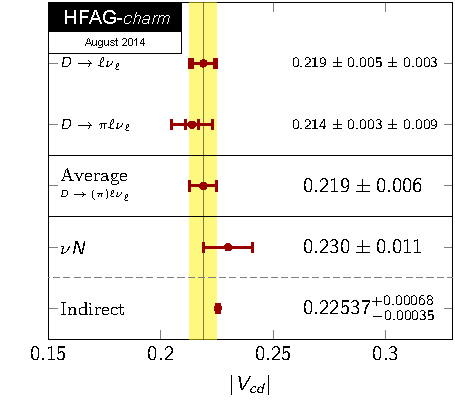
\includegraphics[width=0.49\textwidth]{figures/charm/Vcd.pdf}~
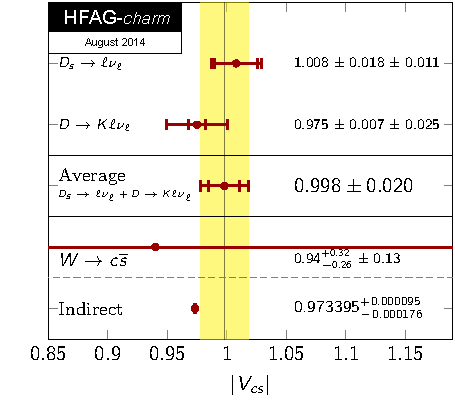
\includegraphics[width=0.49\textwidth]{figures/charm/Vcs.pdf}
\caption{
Comparison of magnitudes of the CKM matrix elements $|V_{cd}|$ (left) and $|V_{cs}|$ (right) determined from the (semi-)leptonic charm decays and from neutrino scattering data
or $W$ decays and indirect determination from the global fit assuming CKM unitarity~\cite{Charles:2004jd}.
\label{fig:VcdVcsComparions}
}
\end{figure}

\subsubsection{Extraction of $D_{(s)}$ meson decay constants}

Assuming unitarity of the CKM matrix, the values of the elements relevant in the case of \mbox{(semi-)leptonic} charm decays are known from the global fit
of the CKM matrix, $|V_{cd}|=0.22537^{+0.00068}_{-0.00035}$, and
$|V_{cs}|=0.973395^{+0.000095}_{-0.000176}$~\cite{Charles:2004jd}. 
These values can be used to extract the $D$ and $D_s$ meson decay constants from the experimentally measured products $f_{D}|V_{cd}|$ (Eq.~\ref{eq:expFDVCD}) and $f_{D_s}|V_{cs}|$ (Eq.~\ref{eq:expFDSVCS}),
respectively. This leads to the experimentally measured $D_{(s)}$ meson decay constants to be:
\begin{eqnarray}
f_D^{\rm exp} & = & (203.7\pm4.9)~{\rm MeV,}\\ 
f_{D_s}^{\rm exp} & = & (257.4\pm4.6)~{\rm MeV,}
\end{eqnarray}
and the ratio of the constants is determined to be
\begin{equation}
f_{D_s}^{\rm exp}/f_D^{\rm exp} = 1.264\pm0.038.
\label{eq:fDsfDRatio:WA}
\end{equation}
The values are in agreement with the LQCD determinations given in Table~\ref{tab:Lattice} within the uncertainties. The largest discrepancy is in the determinations of 
the ratio of the decay constants where the agreement is only at the level of $1.9\sigma$.


\clearpage
\subsection{Hadronic decays of $D_s$ mesons}

\babar, CLEO-c and Belle collaborations have measured the absolute branching fractions of hadronic decays, $\dsp\to K^-K^+\pi^+$, $\dsp\to \overline{K}{}^0\pi^+$, and $\dsp \to \eta\pi^+$. The first two 
decay modes are the reference modes for the measurements of branching fractions of the $\dsp$ decays to any other final state. Table \ref{tab:DSExpHadronic} and 
Fig.~\ref{fig:DSExpHadronic} summarise the individual measurements and averaged values, which are found to be 
\begin{eqnarray}
\br^{\rm WA}(\dsp\to K^-K^+\pi^+) & = & (5.44\pm0.14)\%,\\
\br^{\rm WA}(\dsp\to \overline{K}{}^0\pi^+) & = & (3.00\pm0.09)\%,\\
\br^{\rm WA}(\dsp\to \eta\pi^+) & = & (1.71\pm0.08)\%,
\end{eqnarray}
where the uncertainties are total uncertainties. 

\begin{table}[t!]
\caption{Experimental results and world averages for branching fractions of $\dsp\to K^-K^+\pi^+$, $\dsp\to \overline{K}{}^0K^+$, and
$\dsp\to \eta\pi^+$ decays. The first uncertainty is statistical and the
second is experimental systematic. CLEO-c reports in Ref.~\cite{Onyisi:2013bjt}
$\br(\dsp\to K^0_SK^+)$. We include it in the average of $\br(\dsp\to \overline{K}{}^0K^+)$ by using the relation $\br(\dsp\to \overline{K}{}^0K^+)\equiv 2\br(\dsp\to K^0_SK^+)$.
\label{tab:DSExpHadronic}}
\begin{center}
\begin{tabular}{lcll}
\toprule
\rowcolor{Gray} Mode 	& ${\cal{B}}$ ($10^{-2}$)				& Reference 	& \\ 
\midrule
\multirow{3}{*}{$K^-K^+\pi^+$}  & $5.78\pm0.20\pm 0.30$ 		& \babar		& \cite{delAmoSanchez:2010jg}\\ 
						& $5.55\pm0.14\pm 0.13$ 		& CLEO-c		& \cite{Onyisi:2013bjt}\\ 
						& $5.06\pm0.15\pm 0.21$ 		& Belle   		& \cite{Zupanc:2013byn}\\
\midrule
\rowcolor{Gray}$K^-K^+\pi^+$	& $5.44\pm0.09\pm 0.11$			& Average & \\
\midrule
\multirow{2}{*}{$\overline{K}{}^0K^+$}		& $3.04\pm0.10\pm 0.06$ 		& CLEO-c		& \cite{Onyisi:2013bjt}\\ 
								& $2.95\pm0.11\pm 0.09$ 		& Belle   		& \cite{Zupanc:2013byn}\\
\midrule
\rowcolor{Gray}$\overline{K}{}^0K^+$		& $3.00\pm0.07\pm 0.05$			& Average & \\
\midrule
\multirow{2}{*}{$\eta\pi^+$}  	& $1.67\pm0.08\pm 0.06$ 		& CLEO-c		& \cite{Onyisi:2013bjt}\\ 
						& $1.82\pm0.14\pm 0.07$ 		& Belle   		& \cite{Zupanc:2013byn}\\
\midrule
\rowcolor{Gray}$\eta\pi^+$	& $1.71\pm0.07\pm 0.08$			& Average & 
\\ \bottomrule
\end{tabular}
\end{center}
\end{table}
\begin{figure}[hbt!]
\centering
%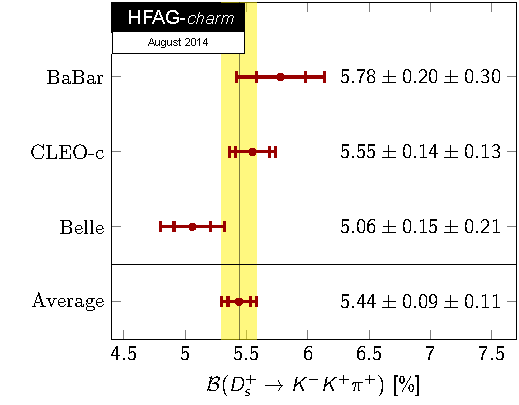
\includegraphics[width=0.325\textwidth]{figures/charm/KKpi.pdf}
%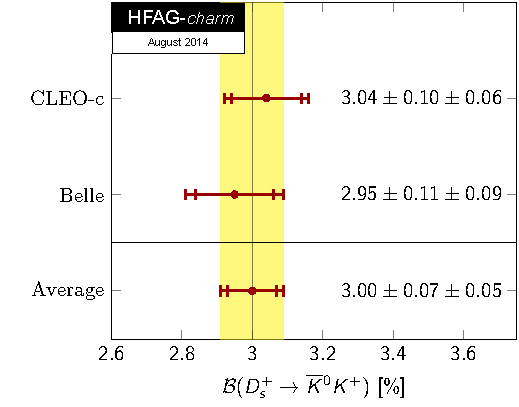
\includegraphics[width=0.325\textwidth]{figures/charm/K0K.pdf}
%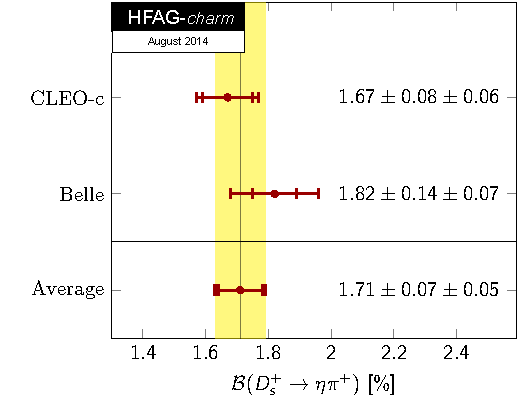
\includegraphics[width=0.325\textwidth]{figures/charm/etapi.pdf}
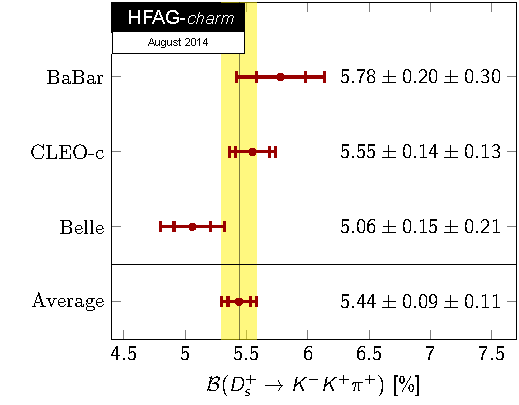
\includegraphics[width=0.50\textwidth]{figures/charm/KKpi.pdf}
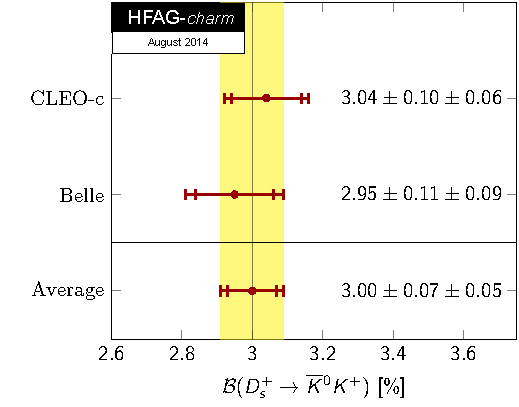
\includegraphics[width=0.50\textwidth]{figures/charm/K0K.pdf}
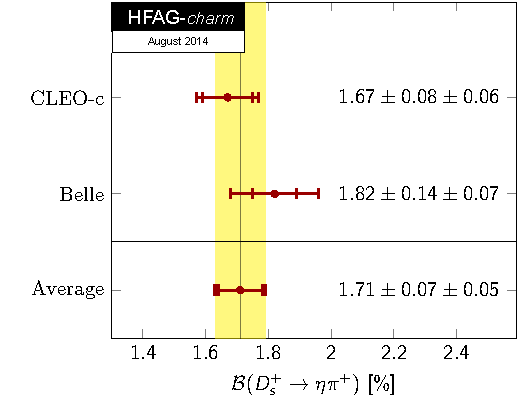
\includegraphics[width=0.50\textwidth]{figures/charm/etapi.pdf}
\caption{
WA values for $\br(\dsp\to K^-K^+\pi^+)$ (top),
$\br(\dsp\to \overline{K}{}^0\pi^+)$ (middle), $\br(\dsp\to \eta\pi^+)$ (bottom).
For each point, the first error listed is the statistical and the second error
is the systematic error.
\label{fig:DSExpHadronic}
}
\end{figure}
